\chapter{Evaluation}
\section{Strong scaling}

\begin{figure}
    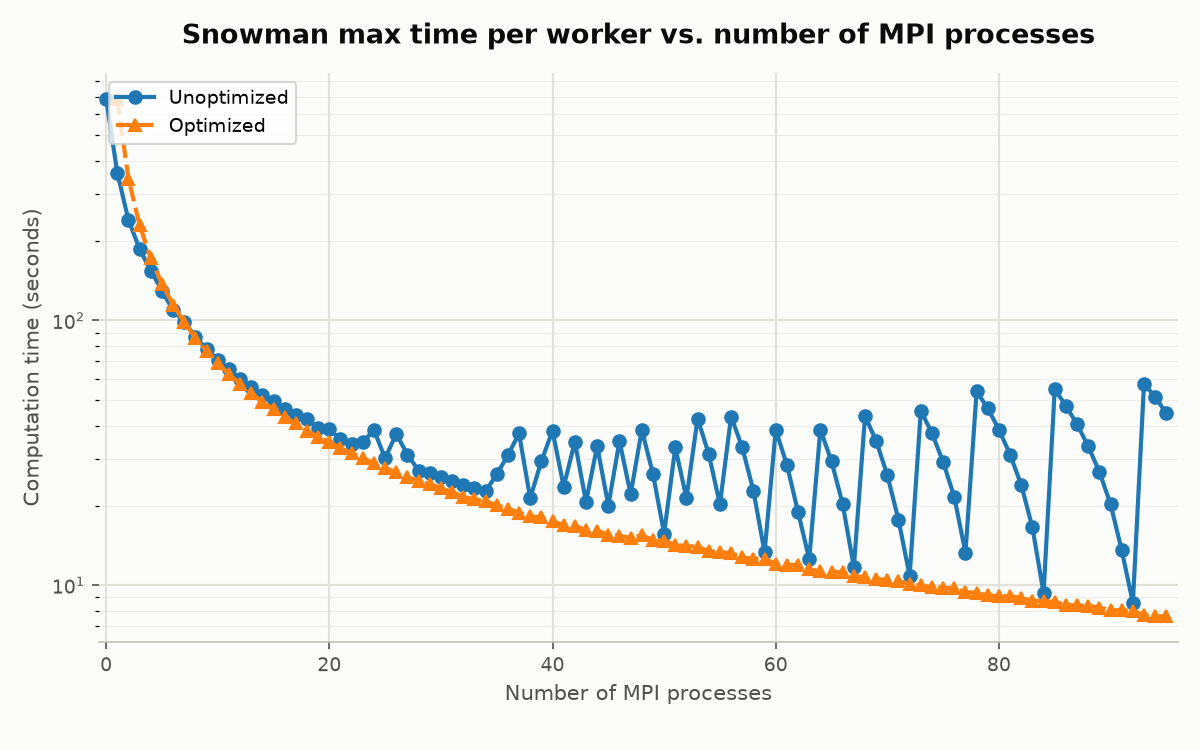
\includegraphics[width=\textwidth]{parts/images/max_times_comparison.png}
    \caption{Runtime for 1 to 96 MPI processes}
\end{figure}

Figure 2.1 shows the runtimes of the optimized and unoptimized code for 1 to 96 MPI processes. A logarithmic scale is used, so differences in the lower runtimes can be seen more clearly. The spikes in runtime of the unoptimized code come from the way the remainder is handled when the rows of the image can not be evenly distributed among the processes: the entire remainder is given to the last process, leading to an uneven distribution of work. Using our tile decomposition, these spikes disappear. This is because the remainder is handled differently. If the image is not evenly divisible by the tile width, the tiles of the image become smaller than the desired tile width. This way the remainder is distributed over multiple processes.\\
\\
We also see that when using few processes, the optimized code is slower. This is because the "master" process is only handling the distribution of the work and is not doing any of the computations to render the image. When using nine or more processes, the optimized code is consistently faster.

\section{Weak scaling}



\section{Comparing different tile sizes}

\begin{figure}
    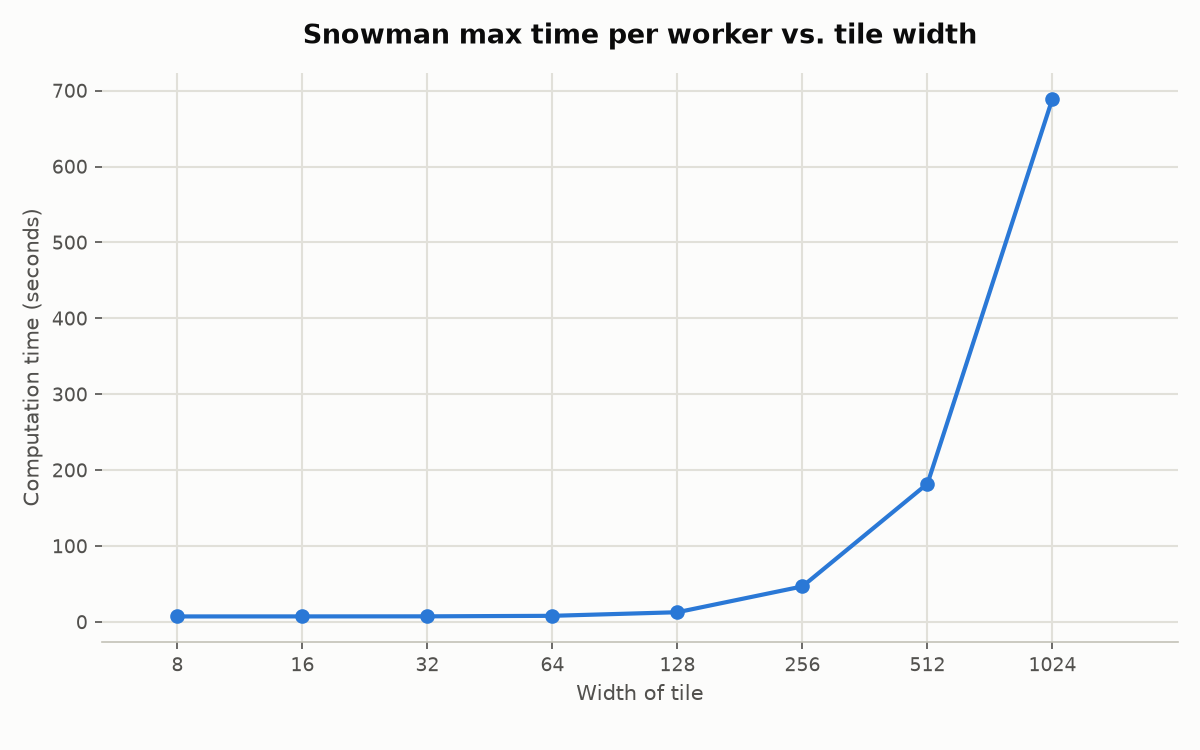
\includegraphics[width=\textwidth]{parts/images/tile_size_ntasks_96.png}
    \caption{Runtime of optimized code on 96 processes for different tile sizes}
\end{figure}

We compared different tile sizes while utilizing a whole node (so 96 workers). The runtime is best for a tile width of 8 pixels (7.31 s) and stays relatively stable up to 64 pixels (8.12 s). The runtime rises dramatically for larger tile sizes. This is to be expected, because there are no longer enough tiles to keep all workers busy. The worst case is a tile width of 1024 pixels (689.52 s). Here, there is just one tile which is the size of the entire image, so the whole image gets processed by one worker. 